% Living project document. Compile with XeLaTeX (twice), or scripts/build_notebook.sh.
% Keep evidence status, experiment IDs, source snapshot, and update log current.
\documentclass[11pt,a4paper]{article}
\usepackage[margin=23mm,headheight=15pt]{geometry}
\usepackage{fontspec}
\setmainfont{Latin Modern Roman}
\setsansfont{Latin Modern Sans}
\setmonofont{Latin Modern Mono}[Scale=0.87]
\usepackage{amsmath,amssymb}
\usepackage{unicode-math}
\setmathfont{Latin Modern Math}
\usepackage{xcolor,booktabs,tabularx,longtable,array,enumitem,fancyhdr}
\usepackage{tikz}
\usetikzlibrary{arrows.meta,positioning}
\usepackage{fvextra}
\usepackage{xurl}
\usepackage[colorlinks=true,linkcolor=blue!45!black,urlcolor=blue!45!black,citecolor=blue!45!black]{hyperref}
\hypersetup{pdftitle={TRM: a living guide to the project},pdfauthor={TRM Decision Stability project},pdfsubject={Evidence, theory, and next experiments}}
\definecolor{ink}{HTML}{15364B}
\definecolor{teal}{HTML}{087E8B}
\definecolor{pale}{HTML}{EFF5F7}
\definecolor{muted}{HTML}{4F606B}
\setlength{\parindent}{0pt}
\setlength{\parskip}{6pt plus 1pt}
\setlength{\emergencystretch}{2em}
\setlist{nosep,leftmargin=1.5em,topsep=5pt,itemsep=3pt}
\renewcommand{\arraystretch}{1.22}
\newcolumntype{Y}{>{\raggedright\arraybackslash}X}
\newcolumntype{P}[1]{>{\raggedright\arraybackslash}p{#1}}
\newcommand{\status}[1]{\par\noindent{\sffamily\small\bfseries\color{teal}#1}\par}
\newcommand{\takeaway}[1]{\par\smallskip\noindent\colorbox{pale}{\parbox{\dimexpr\linewidth-2\fboxsep\relax}{\textbf{What to carry forward.} #1}}\par\smallskip}
\newcommand{\repo}[2]{\href{https://github.com/NiccoGrillo/TinyRecursiveModels/blob/main/#1}{#2}}
\newcommand{\code}[1]{\nolinkurl{#1}}
\newcommand{\Fix}{\operatorname{Fix}}
\newcommand{\norm}[1]{\left\lVert #1\right\rVert}
\newcommand{\newtopic}{\clearpage}
\pagestyle{fancy}
\fancyhf{}
\fancyhead[L]{\sffamily\small\color{muted}TRM \textbar\ Living project guide}
\fancyhead[R]{\sffamily\small\color{muted}6 November 2026}
\fancyfoot[L]{\sffamily\footnotesize Version 1.0 \textbar\ Evidence and hypotheses kept separate}
\fancyfoot[R]{\sffamily\small\thepage}
\renewcommand{\headrulewidth}{0.3pt}
\setcounter{tocdepth}{1}
\begin{document}
\thispagestyle{empty}
{\sffamily\small\color{teal}TRM DECISION STABILITY\hfill LIVING RESEARCH NOTEBOOK\par}
\vspace{12mm}
{\sffamily\Huge\bfseries\color{ink}What we tested,\\[3pt]what we learned,\\[3pt]and what comes next\par}
\vspace{6mm}
{\Large A guide to the project, from the original fixed-point question to the current feedback-timing hypothesis\par}
\vspace{7mm}
\textbf{Snapshot: 6 November 2026.}\quad Version 1.0.\\
Research/code snapshot: \code{8942518}; reported pilot results: \code{98689fb}.\\
Repository: \href{https://github.com/NiccoGrillo/TinyRecursiveModels}{NiccoGrillo/TinyRecursiveModels}.

\section*{Start with these four facts}
\begin{enumerate}
\item \textbf{We have not trained a new model.} We examined frozen, publicly available TRM weights on Sudoku. The main pilot used 32 puzzles; interventions used a nested subset of eight.
\item \textbf{The pilot found late solving, without observed loss of solved answers.} In the longer FP32 run, 25 of 32 puzzles were correct at the usual budget and 27 were correct at the end. None of the 27 ever-solved puzzles became wrong at the logged observation points.
\item \textbf{The new insight is about how two evolving states interact.} Giving the working state more updates before refreshing the answer state can change the stability of their feedback. A mathematical example proves that this can happen. We have not shown that it explains trained TRM.
\item \textbf{The next substantial experiment is ready but has not been run.} It compares two update schedules from identical saved states, on 1,024 new development puzzles, with equal computation budgets. Its result determines whether this direction deserves further work.
\end{enumerate}

\takeaway{The critic accepted a precise, falsifiable question and the mathematical reasoning behind it. This was internal AI review. It was not confirmation that the proposed mechanism occurs in TRM, that a new method works, or that the project is ready for an A* conference.}

\vfill
{\small This document is the human-readable entry point. Read the main sections for the research story; use the appendices for proofs, exact protocols, commands and provenance. The editable source and PDF are maintained together in the repository.}

\newtopic
\section*{How to read and use this guide}
\addcontentsline{toc}{section}{How to read and use this guide}
The text assumes familiarity with neural networks, but introduces the dynamical-systems vocabulary before using it. The symbols in the main explanation are deliberately simple: $h$ is the answer state, $w$ is the working state, and $L$ is the number of working updates before one answer update.

\begin{tabularx}{\linewidth}{@{}P{29mm}Y@{}}
\toprule
Label & Meaning throughout this document\\\midrule
\textbf{Observed} & A result of the trained-checkpoint pilot recorded in the pushed project reports.\\
\textbf{Proved / illustrated} & A mathematical deduction or an explicitly artificial example. It is not a trained-model result.\\
\textbf{Implemented} & Code exists and its behavior has been checked. This does not imply the scientific study has been executed.\\
\textbf{Proposed} & A possible future study or method, conditional on earlier evidence.\\\bottomrule
\end{tabularx}

\textbf{Evidence source.} The empirical numbers below come from the user's committed \repo{docs/STATUS.md}{STATUS.md} and \repo{docs/PILOT.md}{PILOT.md}, including their recorded independent report checks. The raw pilot outputs are not present in this documentation workspace; this document does not claim a fresh reanalysis of those raw records. Mathematical deductions and current source code were checked separately. No new benchmark was run while writing this guide.

\textbf{If you have ten minutes:} read Sections~\ref{sec:story}, \ref{sec:results}, \ref{sec:insight} and \ref{sec:next}. For the meaning of an update, return to Section~\ref{sec:machine}. The appendices are reference material, not prerequisites.

\begingroup
\small
\setlength{\parskip}{0pt}
\makeatletter
\renewcommand{\l@section}[2]{\@dottedtocline{1}{0em}{2em}{#1}{#2}}
\makeatother
\tableofcontents
\endgroup

\newtopic
\section{The research story so far}\label{sec:story}
\subsection*{The question we started with}
The initial intuition was: perhaps requiring a model's entire hidden state to settle to a fixed point is unnecessarily restrictive. Could it keep moving internally while preserving a useful answer? Could ideas about attracting sets, manifolds or stable outputs help?

That is a sensible distinction, but it contains two separate questions. First, \emph{can} an answer stay unchanged while its hidden representation moves? Yes: many different hidden vectors can produce the same decoded answer. Second, \emph{does encouraging this help trained models solve or retain answers?} That needs evidence and comparison with existing approaches. The first observation alone is not a new method.

\subsection*{What we did, in order}
\begin{tabularx}{\linewidth}{@{}P{23mm}Y Y@{}}
\toprule
Date & Work completed & What it changed\\\midrule
4 Nov & Built a TRM adapter, logging, perturbation controls and a small frozen-checkpoint pilot. & Made it possible to continue the same puzzle without resets and branch from the same full state.\\
4--5 Nov & Completed 32-puzzle continuation and eight-puzzle intervention runs. & Found late recovery; did not find the correct-answer loss needed to motivate a retention repair.\\
5 Nov & Compared the protocol with InfiLoop and checked close completion/stability work. & Recognized major differences in checkpoints, update units and observation policies, as well as substantial prior-work overlap.\\
5 Nov & Froze and implemented the larger schedule comparison. & Chose one consequential next test instead of more tiny perturbation sweeps.\\
6 Nov & Developed and critically checked a coupled-feedback example. & Narrowed the possible mechanism: feedback timing can change attraction without deleting an existing fixed point.\\
\textbf{Next} & Run the already specified 1,024-puzzle study. & Determine whether there is a real, useful phenomenon worth explaining or controlling.\\\bottomrule
\end{tabularx}

\subsection*{Where the original idea now stands}
We have \textbf{not} demonstrated a solution manifold, trained an attracting-set model, implemented a new PDE/ODE reasoner, or shown that full-state contraction hurts TRM. The current project uses a discrete recurrent system that already exists. Its immediate question is whether changing \emph{when its two states exchange updated information} changes retention or recovery at equal computational cost.

This preserves the useful part of the original intuition: the whole internal state and the answer need not have identical stability requirements. It also gives us something concrete to intervene on and potentially falsify.

\newtopic
\section{The actual machine: what TRM updates}\label{sec:machine}
\subsection*{One Sudoku, two arrays, one shared network}
For one Sudoku puzzle, TRM stores two arrays of real-valued features. We call them:
\begin{itemize}
\item $h$: the \textbf{answer state}, called \code{z_H} in the code. A small output head reads this array to predict the board.
\item $w$: the \textbf{working state}, called \code{z_L}. It influences future updates of $h$, but is not read directly by the output head.
\end{itemize}
These names describe their computational roles. They do not mean that $h$ literally contains Sudoku digits or that $w$ contains interpretable written reasoning. In the current configurations, each state for one puzzle has shape $97\times512$: 81 cell positions plus 16 prefix positions, each with 512 features. A batch of eight has shape $8\times97\times512$.

Let $x$ denote the fixed input embedding of the puzzle, including the model's positional/prefix information. Let $G$ denote the shared two-block neural module. Ignoring the fixed positional arguments in the notation, the source implements:
\begin{align}
w &\leftarrow G(w+h+x) &&\text{working update},\label{eq:low}\\
h &\leftarrow G(h+w) &&\text{answer update}.\label{eq:high}
\end{align}
\textbf{It is the same $G$ in both equations.} Its parameters are shared. The arguments differ. The actual implementation adds the current state and its injection \emph{before} the shared block stack; this matters when constructing a faithful mathematical example.

\begin{center}
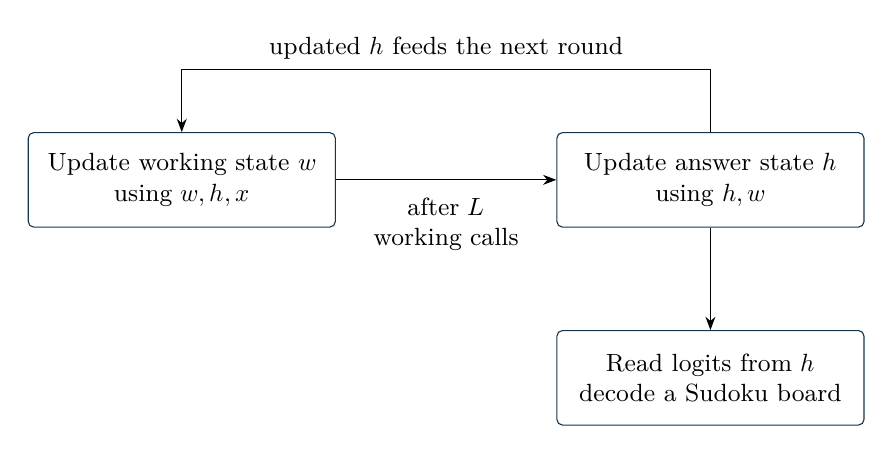
\begin{tikzpicture}[>=Stealth, node distance=12mm,
 box/.style={draw=ink,rounded corners=2pt,align=center,minimum width=39mm,minimum height=12mm,font=\small}]
\node[box] (low) {Update working state $w$\\using $w,h,x$};
\node[box,right=28mm of low] (high) {Update answer state $h$\\using $h,w$};
\node[box,below=13mm of high] (read) {Read logits from $h$\\decode a Sudoku board};
\draw[->] (low) -- node[below=1mm,font=\small,align=center,text width=24mm]{after $L$\\working calls} (high);
\draw[->] (high) -- (read);
\draw[->] (high.north) -- ++(0,8mm) -| node[pos=.25,above,font=\small]{updated $h$ feeds the next round} (low.north);
\end{tikzpicture}
\end{center}

The output head computes scores (\emph{logits}) for each possible cell token from $h$. Taking the largest score at each cell gives the predicted board. Changing $w$ alone therefore leaves the \emph{immediate} logits exactly unchanged. It can still change later logits, because the next answer update uses $w$. That simple fact motivated the first interventions.

\textbf{Code anchor:} \repo{models/recursive_reasoning/trm.py}{models/recursive\_reasoning/trm.py}, especially the reasoning module's additive injection and the inner model's \code{forward}. This description is grounded in that code, alongside TRM~\cite{trm}.

\newtopic
\subsection*{The word ``step'' was hiding three different quantities}
The existing pilot logs use \emph{step} for a native macro-step. The newer theoretical note uses one \emph{outer update}. They are not interchangeable.

\begin{tabularx}{\linewidth}{@{}P{36mm}Y r@{}}
\toprule
Unit & What happens at the native setting & Block calls\\\midrule
One working update & Apply $G$ once to update $w$; hold $h$ fixed. & 2\\
One outer update & Update $w$ six times, then update $h$ once. & 14\\
One native macro-step & Perform three outer updates; emit the normal model output. & 42\\
Normal 16-macro budget & 48 outer updates in total. & 672\\
Long pilot: 64 macros & 192 outer updates in total. & 2,688\\\bottomrule
\end{tabularx}

Here $L=6$ is the number of working updates and $H=3$ is the number of outer updates per macro. Each $G$ call contains two block layers. Thus
\[
\underbrace{(L+1)\times2}_{\text{one outer}}=14,
\qquad
\underbrace{H(L+1)\times2}_{\text{one macro}}=42.
\]
Unless explicitly stated otherwise, every depth in the \emph{completed pilot} sections is a macro count. The future study uses outer counts and block budgets explicitly.

\subsection*{Why we preserve both states and bypass resets}
The full continued computation depends on $(h,w)$, the input and the update phase. Copying only $h$ does not produce an identical future computation. Our branches copy both arrays at a specified boundary and keep the puzzle fixed.

The standard ACT wrapper can halt an example and reset its state for subsequent processing. That is appropriate for ordinary operation, but would interrupt a long-trajectory experiment. Our adapter continues the same internal state without those resets. It preserves the underlying recurrence. It does not train new parameters or silently replace pretrained weights with random ones.

\subsection*{What training does, and what this project does}
The upstream model is supervised with target answers at macro outputs and uses a learned halting-related $Q$ head. Within a macro, early outer iterations run without gradients; gradients pass through the final outer iteration, and carried states are detached before the next macro. This is a training-memory choice, not a proof of convergence. The initial-state vectors are checkpoint-stored buffers.

Our current experiments freeze the pretrained weights. Ground-truth boards are used \emph{afterward} to measure correctness, not to choose a branch, perturbation direction or schedule. A Sudoku rule checker tests validity using the puzzle's constraints; that is distinct from inspecting the reference solution.

\takeaway{More working updates means more calls using an unchanged answer state. Reading intermediate outputs only observes the computation; changing the number of working updates changes the computation itself.}

\newtopic
\section{Fixed points, stable answers and moving states}\label{sec:background}
\subsection*{A fixed point need not be unique}
Write $s=(h,w)$ for the full internal state, and $F$ for a complete update rule. A fixed point satisfies $F(s_*)=s_*$. If the model reaches that exact state, the next update leaves it unchanged. The equation may have no solutions, one solution, or many solutions. ``Fixed point'' by itself does \emph{not} mean ``one unique representation for every answer.''

An \textbf{attracting} fixed point also draws nearby states toward it. Its \textbf{basin} is the collection of starting states that eventually approach it. These are different questions: a useful state can exist but be difficult to reach; an incorrect state can be attracting.

\subsection*{The output is a coarse view of the state}
Let $D(h)$ be the board decoded from $h$. The states producing one board $y$ form the set
\[
\mathcal S_y=\{(h,w):D(h)=y\}.
\]
This set can be large because $w$ is not directly read, and many different $h$ vectors have the same largest logit at each cell. The set need not be a smooth \emph{manifold}. A manifold is a set that locally looks like a lower-dimensional continuous space; proving that property requires more than observing unchanged predictions.

Staying in $\mathcal S_y$ means retaining the same decoded board. It does not mean $s$ has stopped. It also does not mean $y$ is correct. A collection of hidden representations of one solution is distinct from a puzzle having several valid solutions.

\subsection*{A small example of the original intuition}
Consider a purely illustrative continuous-time system, with state $(r,\theta)$:
\[
\dot r=-(r-1),\qquad \dot\theta=1\pmod{2\pi}.
\]
The radius approaches 1 while the angle keeps rotating. The attracting object is a circle, not a stationary point. A readout that depends only on the limiting radius could settle while the full state keeps moving. This explains why attraction to a set is a coherent idea; it is not a model we have trained or evidence that TRM uses a circular representation.

In dynamical-systems language, \textbf{transverse stability} concerns disturbances away from such an orbit or set; motion along it can remain. \textbf{Output contraction} asks for readout differences to shrink, a weaker requirement than shrinking every state difference. \textbf{Partial contraction} concerns selected relations or components. These concepts motivate what to measure, but transferring their guarantees requires checking their assumptions~\cite{partial,transverse,output}.

\takeaway{The original point-versus-set question remains meaningful. Our experiments have not identified a manifold or proved any contraction property. The current direction focuses on the coupled update rule that moves the state, because that is something we can directly manipulate.}

\newtopic
\section{The experiment ledger: what actually exists}\label{sec:ledger}
These IDs are stable references for this notebook. They are not new runs. All completed trained-model experiments used the same third-party MLP checkpoint, with the eight-puzzle cohorts nested inside the 32-puzzle cohort.

{\small
\begin{tabularx}{\linewidth}{@{}P{14mm}P{22mm}Y Y@{}}
\toprule
ID & Status & Question / setup & Result or next decision\\\midrule
E0 & Checked & Adapter, zero controls, manifests, strict checkpoint loading, synthetic smoke tests. & Instrumentation evidence; synthetic accuracies are not research results.\\
E1a & Observed & 32 puzzles; native BF16; 16 macros. & 25/32 correct at the endpoint. No correct-to-wrong transition at logged macros.\\
E1b & Observed & Same 32; FP32; continue to 64 macros. & 25/32 correct at 16, 27/32 at 64. No logged loss after solving.\\
E2 & Observed control & Eight puzzles; fork at macros 4, 8, 16; zero perturbation; 16-macro branches. & All 1,152 branch records exactly matched the natural continuation.\\
E3 & Observed & Same eight; perturb only $w$ by 1\% relative norm; random and gradient directions. & Immediate logits unchanged. Some wrong trajectories changed; no correct-at-fork answer was lost.\\
E4 & Implemented; not run & 1,024 new dev puzzles; two checkpoints, two precisions; equal-budget $L=6$ versus $L=12$. & The next scientific result we need. See Section~\ref{sec:next}.\\
T0/T1 & Proved / checked & Original transient example (T0), then shared-core feedback example (T1). & Possibility examples, not tests of trained networks.\\
E5 & Proposed only & If justified by E4: equal numbers of working and answer updates, differently interleaved. & No real-model launcher or outcomes for this follow-up yet.\\\bottomrule
\end{tabularx}}

\subsection*{Why this table matters}
There are four completed main pilot runs, not dozens of independent datasets. Repeating several branches on the same puzzle is useful for paired comparisons, but does not multiply the number of independent puzzles. The eight examples are exploratory and unusually small for a research claim.

The current suite has \textbf{39 passing software/mathematical tests}, recorded at the research snapshot. They check things such as correct state copying, report completeness, budget accounting and finite-difference agreement. They are not 39 successful research experiments. Strict loading of the attention weights and agreement between native and densely observed recurrence establish implementation compatibility, not Sudoku performance.

No FPRM or InfiLoop backend has been implemented in this repository. No learned stabilizer, new training loss or adaptive scheduling controller has been trained or evaluated.

\newtopic
\section{What the natural-continuation pilot tells us}\label{sec:results}
\status{OBSERVED: E1a and E1b. Depths on this page are native macro-steps.}
\begin{tabularx}{\linewidth}{@{}Y c c c@{}}
\toprule
Run & Correct at 16 & Correct at end & Ever-correct then lost\\\midrule
BF16, stop at 16 & 25/32 & 25/32 & No observed losses\\
FP32, continue to 64 & 25/32 & 27/32 & 0/27 puzzles\\\bottomrule
\end{tabularx}

\subsection*{Follow the same puzzles, rather than just the percentages}
At FP32 macro 16, 25 puzzles were correct and seven were wrong. By macro 64:
\begin{itemize}
\item all 25 initially correct puzzles were still correct and had stayed correct at every logged macro;
\item two of the seven initially wrong puzzles had become correct;
\item five were still wrong at the endpoint.
\end{itemize}
Accuracy therefore rose from 78.125\% to 84.375\%, an improvement of 6.25 percentage points. The reported paired puzzle-bootstrap 95\% interval was $[0,15.625]$ percentage points. This is a small exploratory sample, not a precise population estimate.

\subsection*{``No observed loss'' has a specific scope}
Outputs were logged after each native macro, not after every answer update inside it. A board could have become wrong between two logged outputs and recovered before the next one. E1b therefore establishes no observed loss on its \emph{macro observation grid}. It does not establish permanent correctness or stability at every internal update.

The reports list 0/334 and 0/1,608 correct-to-wrong transitions for BF16 and FP32 respectively. Those many transitions reuse the same puzzles; they are correlated. They should not be described as hundreds or thousands of independent examples. For continuation from the usual budget, the useful count is 0/25 FP32 puzzles losing correctness through macro 64.

\subsection*{Precision changes more than the final aggregate score}
Both runs achieved 25/32 at macro 16, but not on exactly the same puzzles: one was correct only in BF16 and another only in FP32. Full predicted boards matched on 24/32 puzzles. BF16 uses lower-precision arithmetic than FP32; equal aggregate accuracy does not imply identical trajectories.

We have \textbf{not} measured BF16 continuation beyond macro 16 in this pilot. It would be incorrect to use the FP32 extension as evidence about every numerical regime. The run times also overlapped, so their recorded wall times are not a controlled speed comparison.

\takeaway{The pilot gave us a recovery phenomenon, not the retention failure we initially expected to repair. That is why the project did not proceed directly to training a stabilizer.}

\newtopic
\section{What the perturbation experiment changed}\label{sec:perturb}
\status{OBSERVED: E2 and E3. A sensitivity experiment, not an inference method.}
\subsection*{The intervention, step by step}
At each predetermined macro (4, 8 or 16), we saved the same $(h,w)$ and made several copies. One copy continued unchanged. In the others we replaced $w$ with $w+\delta$, keeping $h$ untouched. The nonzero intervention was chosen so that
\[
\frac{\norm{\delta}}{\norm{w}}\simeq0.01.
\]
In plain terms, the change had about 1\% of the working state's norm. Since the current output depends only on $h$, all immediate logits had to remain identical. That equality was explicitly checked, rather than assumed from an approximate similarity score.

\textbf{Random $+$ and $-$} use opposite directions along a random perturbation. \textbf{Gradient $+$ and $-$} use opposite directions derived from a short future-margin objective. The margin compares the score of the model's current predicted token with alternatives; the probe uses current predictions, not the reference answer. Gradient plus follows the direction that locally reduces that future margin; minus reverses it. A two-macro lookahead and backward pass cost extra computation. Neither sign guarantees better or worse correctness.

All branches then continued for 16 macros, beyond the two-macro gradient probe. We compared each branch with the matching clean continuation at the same offset. We did not search for a favorable fork after looking at labels.

\subsection*{First, the zero control}
E2 set $\delta=0$. All 1,152 branch records matched the corresponding natural trajectory, including predictions and logged observables. This validates copying and continuation. It is not evidence that perturbations help.

\subsection*{Then, the nonzero result}
At every fork, five of the eight puzzles were correct and three were wrong. All 96 nonclean puzzle/fork/arm interventions met the norm tolerance and preserved immediate logits exactly.

{\small
\begin{tabularx}{\linewidth}{@{}c Y c c c@{}}
\toprule
Fork & Arm(s), each separately & Final solve & Loss from correct & Recovery from wrong\\\midrule
4 & Random $\pm$, gradient $\pm$ & 6/8 & 0/5 & 1/3\\
8 & Gradient $+$ & 5/8 & 0/5 & 0/3\\
8 & Random $\pm$, gradient $-$ & 6/8 & 0/5 & 1/3\\
16 & Random $\pm$, gradient $\pm$ & 6/8 & 0/5 & 1/3\\\bottomrule
\end{tabularx}}
The clean final solve count was 6/8. Grouped arms above share the same numerical result; they are not pooled samples. No correct-at-fork puzzle changed its board relative to clean at any observed branch offset.

\newtopic
\subsection*{One actual puzzle makes the distinction concrete}
One puzzle, with ID beginning \code{e524867c}, was wrong at all three forks. Its clean trajectory first became correct at macro 17. Under the gradient-plus intervention:

\begin{tabularx}{\linewidth}{@{}P{35mm}Y Y@{}}
\toprule
Continuation & What happened & Meaning\\\midrule
No intervention & First correct at macro 17. & The usual 16-macro budget had stopped just before recovery.\\
Perturb at macro 4 & First correct at macro 7. & Recovery was accelerated in this example.\\
Perturb at macro 8 & Still wrong at branch endpoint, macro 24. & Recovery was prevented or delayed beyond the measured window.\\
Perturb at macro 16 & First correct at macro 17. & The measured solve time was unchanged.\\\bottomrule
\end{tabularx}

This is \textbf{not} a case where a correct solution was destroyed. At macro 8 the answer was already wrong. The intervention changed whether it became correct later. Nor does failure through macro 24 prove that it would never recover.

The final eight-puzzle gradient-plus difference at fork 8 was $-12.5$ percentage points, with a reported pointwise 95\% bootstrap interval of $[-37.5,0]$. With one changed outcome and only eight examples, this does not establish a reliable stage-dependent law. Other perturbation directions sometimes accelerated the same puzzle too. The case was selected for inspection after the results were known.

\subsection*{The narrow conclusion that is supported}
Changing information not read by the current output can change later answers. That is evidence that \emph{present readout equivalence does not imply future dynamical equivalence}. A direction invisible to the current output is not necessarily irrelevant to the computation.

This experiment did not establish a useful learned controller, spontaneous failure mechanism, stable solution manifold, or successful retention repair. It also did not show that gradient directions are systematically better than random directions.

\subsection*{Why not simply do more of the same?}
The desired practical motivation was to preserve already correct answers. Neither natural continuation nor these perturbations exposed that failure in the tested cohort. Stronger attacks could manufacture failures without explaining normal behavior. Close prior work also already studies late completion and directional stability~\cite{finish}. The next useful experiment should address the unresolved protocol and dynamics questions at a substantial scale.

\takeaway{``An intervention changed future correctness'' is the observed fact. ``We identified and repaired the cause of overthinking'' would be an unsupported interpretation.}

\newtopic
\section{Why the project changed direction}\label{sec:shift}
\subsection*{The apparent disagreement with InfiLoop}
InfiLoop v2 reports a TRM retention problem: its Figure 1 shows 19.7\% solved-puzzle loss after 36 additional outer updates. The cohort contains puzzles both compared models solve within the initial 36 updates. A separate 20.9\% statistic concerns cells, not whole solved puzzles~\cite{infiloop}.

Our pilot did not replicate that setup:

\begin{tabularx}{\linewidth}{@{}P{33mm}Y Y@{}}
\toprule
Dimension & Our longer pilot & InfiLoop diagnostic\\\midrule
Model & Third-party MLP TRM & Self-attention TRM\\
Observation & One readout per three outer updates & Outer-update readouts\\
Cost per outer & 14 block layers & 26 block layers\\
Precision & FP32 continuation & Exact figure precision not verified\\
Cohort & 32 predetermined dev puzzles & Jointly solved cohort of two models\\\bottomrule
\end{tabularx}

We inspected the released code and relevant figure text, but did not identify the exact Figure-1 TRM checkpoint and complete reproduction script. The pilot neither reproduces nor refutes that figure. Its 64 macros already cost 2,688 block evaluations, so ``we simply did too little total computation'' is not an established explanation.

\subsection*{Observation frequency and update schedule are different interventions}
Suppose a native trajectory emits correct boards at macros 16 and 17. Looking between those outputs might reveal an incorrect intermediate board. We have learned something by observing more often, but we have not changed the model and have not shown failure of its usual output policy.

By contrast, changing $L$ from 6 to 12 inserts six extra working updates before each answer refresh. It changes the path of the computation. Matching the other paper's 26-block cost this way is \emph{not} an exact reproduction of its checkpoint or training schedule.

\subsection*{The literature also narrowed the available claim}
\emph{When Recursive Models Finish Computing} studies extended TRM recurrence, directional stability and perturbations, including the same MLP checkpoint. FPRM Appendix F already investigates inner/outer compute allocation. TAPS already adapts update strength~\cite{finish,fprm,taps}. A small perturbation study or a schedule accuracy table would be insufficient on its own.

\takeaway{We chose a controlled schedule comparison to distinguish observation effects, numerical/checkpoint effects and continuation-schedule effects. A positive result would still need a predictive mechanism and a useful intervention to support a new method.}

\newtopic
\section{The new insight, explained before the algebra}\label{sec:insight}
\status{HYPOTHESIS ABOUT TRM; SUPPORTED BY A MATHEMATICAL POSSIBILITY EXAMPLE}
\subsection*{The intuition: local improvement can worsen the feedback}
During working updates, $w$ repeatedly uses the same held-fixed $h$. Then $h$ changes using the resulting $w$. More working updates may make $w$ better adjusted to the \emph{old} $h$, while making the next change of $h$ larger or badly coordinated with the coupled system.

Think of $h$ as a current proposal and $w$ as working notes tied to that proposal. Refining the notes for longer need not help if the next proposal update changes what those notes should be responding to. This is an analogy for the equations, not a claim that the features are interpretable notes.

The hypothesis is therefore: \textbf{some limits of continued reasoning may depend on the timing and strength of feedback between the two states, even when the same exact fixed states remain available.} We have not yet shown this mechanism in a trained network.

\subsection*{Existence and attraction are separate: a one-number example}
Both rules below have the fixed point $s_*=0$:
\[
s_{t+1}=0.5s_t,
\qquad\qquad
s_{t+1}=1.2s_t.
\]
Starting at 0.1, the first gives $0.1,0.05,0.025,\ldots$; the second gives $0.1,0.12,0.144,\ldots$. The fixed point has not disappeared. Nearby states simply move differently. Starting at \emph{exactly} zero stays at zero under either rule.

The current TRM question has this same logical structure, with a high-dimensional coupled state. We ask whether changing the update schedule can preserve a state that solves the fixed-point equation while changing whether nearby trajectories approach it.

\subsection*{What we can prove for TRM's update structure}
Call one working-only update $A$ and one answer-only update $B$. One outer update with $L$ working calls is
\[
F_L=B\circ A^L.
\]
Here $A^L$ means apply $A$ repeatedly $L$ times, then apply $B$. Since $A$ leaves $h$ unchanged and $B$ leaves $w$ unchanged, any exact fixed point of $F_6$ is also an exact fixed point of $F_{12}$. Appendix~\ref{app:proofs} gives the short proof.

This result says \emph{nothing} about correctness, attraction, the basin, or behavior from ordinary finite-budget states. It also concerns one outer update; a state fixed after a three-outer macro could instead be part of a three-cycle.

\newtopic
\subsection*{A concrete coupled example: same solution, different stability}
We constructed an artificial scalar system with TRM's shared additive wiring:
\[
G(v)=v(v-1)(0.7v+0.2),\qquad x=1,
\]
\[
w\leftarrow G(w+h+1)\quad L\text{ times},\qquad
h\leftarrow G(h+w).
\]
It uses one number for each state instead of a large array. At $(h,w)=(0,0)$, both updates return zero. Each subsystem is locally stable when the other state is held fixed. Nevertheless:

\begin{tabularx}{\linewidth}{@{}Y c Y@{}}
\toprule
Schedule & Local growth factor & What happens near the origin\\\midrule
$L=6$ & 0.670489 & Nearby errors eventually shrink.\\
$L=12$ & 1.254233 & An error direction grows.\\
$L=12$, damp answer update to 80\% & 0.694608 & Local attraction is restored.\\\bottomrule
\end{tabularx}
The displayed factor is the \emph{spectral radius}: the largest magnitude of the linearized update's eigenvalues. Below one means local asymptotic attraction here; it does not mean every single step decreases every error norm. Appendix~\ref{app:toy} derives the values and damping threshold.

Damping means taking only part of the proposed answer-state change:
\[
h_{\mathrm{new}}=h+\eta\bigl(h_{\mathrm{proposal}}-h\bigr).
\]
For example, $\eta=0.8$ accepts 80\% of the proposed change. Damping is a standard idea and an essential baseline, not the claimed novelty.

\subsection*{What the critic accepted, and what it did not}
The critic required the example to use \emph{one shared function with additive inputs}, matching the actual code's wiring. An earlier, more general construction did not meet that constraint and was rejected. The corrected example and fixed-set argument survived review. They provide a reason to test a coupled-feedback explanation.

They do not construct actual post-normalized Transformer weights, demonstrate a trained-model instability, identify ODE stiffness, or show that a latent instability changes a discrete Sudoku answer. A scalar existence example is not a performance result.

\textbf{A hard limit:} timing alone cannot move an exact state fixed by both $A$ and $B$. If that state decodes incorrectly, repeating or damping those unchanged updates still leaves it there. A constant wrong board, however, is not proof of an exact latent fixed point.

\takeaway{The surviving idea is a causal account of coupled feedback, with a useful intervention predicted in advance. The mathematical example establishes possibility. E4 must establish whether there is a relevant trained-model effect to pursue.}

\newtopic
\section{The next experiment, with every comparison spelled out}\label{sec:next}
\status{E4: IMPLEMENTED; FULL TRAINED-CHECKPOINT STUDY NOT YET RUN}
\subsection*{The question}
From the same state reached by normal TRM computation, does changing the balance of working updates and answer updates alter retention or recovery, when both continuations get the same block budget?

\subsection*{For each puzzle, do exactly this}
\begin{enumerate}
\item Run the native model for 16 macros: 48 outer updates, or 672 block evaluations. This prefix is shared by the two branches.
\item Save \emph{both} states $(h,w)$ at that fixed boundary. The fork time is predetermined, not the first time a reference answer happens to be correct.
\item Make two identical copies. Continue one with $L=6$ and the other with $L=12$. Keep weights and input fixed; add no perturbation and perform no training.
\item Give \emph{each} continuation 2,184 block evaluations. Log a board after every answer update, and retain separate records of native macro boundaries.
\item After the run, use labels to measure what happened. Correct-at-fork puzzles measure retention; wrong-at-fork puzzles measure recovery.
\end{enumerate}

\begin{tabularx}{\linewidth}{@{}Y c c@{}}
\toprule
Continuation quantity & $L=6$ & $L=12$\\\midrule
Block calls per outer update & 14 & 26\\
Outer / answer updates in branch & 156 & 84\\
Working updates in branch & 936 & 1,008\\
Total branch block calls & 2,184 & 2,184\\
Common-grid spacing & 13 outer updates & 7 outer updates\\\bottomrule
\end{tabularx}

This is an equal-cost \emph{schedule} comparison. It does not isolate just one variable such as the number of working calls: the number of answer refreshes also changes. Within a checkpoint, each shared block has the same shape. Equal block counts are not a claim of equal FLOPs between the MLP and attention architectures, nor equal wall-clock time. Readout and embedding costs are counted separately.

The common grid is every 182 blocks. Intermediate grid points can lie between native macro outputs. At the final budget, both branches have completed a multiple of three outer updates, so their endpoint phases align.

\newtopic
\subsection*{Which puzzles and models?}
Use the same 1,024 project-development puzzles in all four conditions, beginning at offset 32 to exclude the exploratory prefix. The split seed is zero. Conditions are the MLP and attention checkpoints, each in BF16 and FP32. Attention/BF16 is the prespecified primary condition.

Each numerical condition computes its own native prefix. The two branches \emph{within} that condition share the exact state. Cross-precision comparisons do not start from identical latents. With one checkpoint per architecture, architecture and training/checkpoint differences cannot be separated.

\subsection*{Three kinds of ``losing a solution''}
\begin{enumerate}
\item \textbf{Native output loss:} a correct board at a native macro is followed by a wrong board at a later native macro. This concerns the model's usual output policy.
\item \textbf{Intermediate excursion:} after a correct native output, a dense intermediate readout becomes wrong. If every later macro in the window stays correct, ordinary macro logging would miss that excursion.
\item \textbf{Dense first-solve loss:} after the first correct readout at any outer update, a later dense readout becomes wrong. This can include a fleeting intermediate solution never emitted as a native macro output.
\end{enumerate}
These are not interchangeable denominators or claims. The fixed-fork schedule comparison uses the same correct-at-fork cohort in both arms, before either treatment has an outcome. We never select just the puzzles an arm later solves.

There is also a descriptive native observation audit: follow the first eligible native solve for 36 further native outer updates, requiring a complete window. That costs 504 blocks. It is not the 36-times-26-block window of the InfiLoop figure. Late or never-solving puzzles excluded from this audit must be reported.

\subsection*{What is measured and how it will decide the next step}
The primary effect is $L=12$ minus $L=6$ in the fraction of correct-at-fork puzzles that become wrong at \emph{any dense observation}. The prespecified practically meaningful harm is two percentage points. Appendix~\ref{app:stats} explains the paired uncertainty calculation.

Secondary outcomes include final correctness, recovery from wrong-at-fork states, native macro-output loss, and the fraction of the block budget during which the current answer is incorrect. The last statistic holds the most recent $h$ readout constant while the next computation runs; the terminal output has zero duration. It is a computation-budget statistic, not a wall-clock user experience measure.

The sample size is fixed. At least 300 correct-at-fork puzzles is an adequacy flag, not permission to keep collecting until a favorable answer appears. The full four-condition design costs 20,643,840 sample-block evaluations, excluding output heads, input embeddings and analysis.

\newtopic
\section{How results will change the research plan}\label{sec:decisions}
\begin{tabularx}{\linewidth}{@{}P{68mm}Y@{}}
\toprule
Possible E4 outcome & Consequence\\\midrule
The primary 95\% lower bound is above $+2$ percentage points. & Support a practically meaningful harmful schedule effect in this setting. Replicate before assigning a mechanism.\\
The primary upper bound is below $+2$ percentage points. & Exclude that prespecified harmful effect size under this protocol. Do not keep the claim alive by strengthening attacks.\\
The interval includes $+2$ percentage points. & Inconclusive about the target effect size, even if the estimate differs from zero.\\
Intermediate errors occur, but native macro outputs retain correctness. & An observation-frequency finding. This alone does not motivate repairing native output retention.\\
$L=12$ damages answers while native $L=6$ stays stable. & Altered-schedule fragility. It is not evidence that native TRM already has this defect.\\
Both schedules retain answers with informative bounds. & Stop this retention-repair direction for these conditions.\\
A schedule improves final correctness or recovery at equal cost. & Consider a useful allocation method; require a label-free policy and strong baselines.\\\bottomrule
\end{tabularx}

\subsection*{The conditional E5 follow-up: same amounts, different order}
If E4 provides a reason, compare repeated pairs $(6,6)$, $(3,9)$ and $(9,3)$ of working-update counts. In all cases, a pair contains 12 working calls and two answer calls. Repeating 78 pairs gives each arm 936 working updates, 156 answer updates and 2,184 block calls. This controls the number of answer refreshes that differs in E4.

The scalar example predicts a better eventual linearized convergence rate for uneven allocation, but also warns that short-term amplification can be worse. Reversing $(3,9)$ to $(9,3)$ changes the starting phase; it does not change the eigenvalues of the linearized period map. A difference between those arms would need a phase/transient/nonlinear explanation. E5 is not yet part of the trained-model launcher.

\subsection*{What would make this a serious research contribution?}
A mechanism should predict which states benefit, or predict a component-specific damping rescue, \emph{before} seeing their continuation. It must outperform simple fixed schedules, extra native continuation, ordinary damping, TAPS and verifier stopping where applicable, with all diagnostic and search compute charged. It then needs new puzzles and checkpoints beyond those used to design it.

If the only effect is damage from schedules the model never trained on, we have not produced a useful method. A toy and a schedule sweep do not establish conference-level novelty. Stopping an unsupported line is part of the plan.

\newtopic
\section{How the papers fit together}\label{sec:papers}
These are orientation notes, not interchangeable claims of full reproduction. The project reviewed the closest work to narrow the question; it has implemented only a TRM experimental backend.

\subsection*{The three starting architectures}
\textbf{TRM~\cite{trm}} repeatedly uses a small shared network to update two latent states. It supplies our actual code and frozen checkpoints. It does not enforce a globally contractive fixed-point equation. Our question concerns what happens when that learned recurrence continues or its schedule changes.

\textbf{Fixed-Point Reasoners / FPRM~\cite{fprm}} uses architectural choices including residual scaling and a convergence-based halting mechanism to support deep looping. Its theoretical sufficient conditions should not be confused with unconditional guarantees about every learned checkpoint. Appendix F already compares inner/outer allocation at approximately fixed compute. Thus ``more inner computation can be worse'' is not a new general observation.

\textbf{InfiLoop~\cite{infiloop}} retains a weighted running summary of past recurrent states rather than relying only on the latest proposal. Its memory mechanism motivates examining retention, but it introduces persistent aggregation state that must be included in any faithful dynamical description. Its Figure-1 protocol differs materially from ours, as Section~\ref{sec:shift} explains. We have not reproduced its baseline figure.

\subsection*{The work that most directly limits our novelty}
\textbf{When Recursive Models Finish Computing~\cite{finish}} examines extended recurrence and directional stability on 1,000 Sudoku puzzles, including our MLP checkpoint. It separates unfinished computation from persistent failure. We cannot claim generic late recovery, perturbation sensitivity or directional stability as our new contribution. The project's full-text review was central to choosing a more specific next question.

\textbf{TAPS~\cite{taps}} adapts update scaling using trajectory information. Its update definition and inner/outer control and refresh choices were inspected; the nested recurrence remains. A new timing/feedback controller would need to compare against it. Its code still requires inspection before implementing a fair comparator.

\textbf{QRR~\cite{qrr}} studies convergence after identifying a symmetry in the latent state: hidden motion can continue while the relevant quotient representation settles. \textbf{Invariant-Measure Reasoners / ImR~\cite{imr}} instead reads a prediction through an expectation under a stable distribution. These occupy versions of the original ``stable answer without a stationary hidden state'' idea. ImR's primary abstract was reviewed; a detailed implementation comparison remains open.

\takeaway{The possible contribution is not ``loops can move without changing the answer'' or ``allocation matters.'' It would be a predictive explanation of coupled feedback in trained reasoners, tied to a useful intervention at matched cost.}

\newtopic
\subsection*{Other comparators and dynamical-systems tools}
\textbf{Readout Feedback / RoFB~\cite{rofb}} introduces feedback from intermediate readout probabilities into recurrent dynamics. \textbf{Input-Conditioned Search / ICS~\cite{ics}} changes the input conditions used by the update map. Both matter if we move toward steering wrong trajectories. The project has checked RoFB's introduction/method overview and ICS's primary abstract; their detailed methods and theoretical assumptions still need review.

\textbf{Learning to Compute Is Not Learning to Retain or Reuse~\cite{retain}} separates these abilities through state interventions. Retention failure and causal interventions are therefore not new categories introduced by this project. Random depth/position supervision is a relevant training baseline if training is later justified.

\textbf{Transient amplification~\cite{transient,trefethen}} explains how a system that eventually contracts can first magnify disturbances. Matrices whose directions interact can have this behavior; eigenvalues alone do not measure every short-term change. The distinction matters because we care about finite-budget answers, not only asymptotic convergence.

\textbf{Coupled PDE solvers~\cite{spenke,sheehan}} offer a useful analogy: solving one component more accurately while holding information from another component fixed does not automatically improve the joint iteration. The mathematical precedent is grounding for our hypothesis, not a new numerical-analysis theorem or evidence about TRM weights.

\textbf{Partial, transverse and output contraction~\cite{partial,transverse,output}} formalize different quantities that might stabilize without requiring every coordinate to stop. They are potential theoretical tools for a later result. No metric or bound satisfying those theories has been established for our checkpoints.

\subsection*{Directions being kept in reserve}
A learned schedule, high-state damping, a readout-preserving stabilization loss, attracting-set training or a state-displacing escape mechanism are possible later branches. None is the immediate experiment. Exact common fixed states cannot be escaped by timing alone; adding a new feedback signal or changing the map would be a different intervention and would require the relevant comparators.

The broader resource index also covers DEQs, path independence, normalization/gain control, stochastic stopping, probabilistic TRM, attractor models and torus networks. Those are reading leads rather than results of this project. The maintained full index is \repo{docs/RESOURCES.md}{docs/RESOURCES.md}; it records review depth and source links so incomplete paper review is not mistaken for established novelty clearance.

\newtopic
\section{Keeping this notebook useful as research progresses}\label{sec:living}
\subsection*{The next concrete action}
Run E4 using its frozen settings, preserve the raw records and manifests, and independently regenerate each report. Then update the ledger, result tables and decision section before proposing a new model. The implementation and launch commands are in Appendix~\ref{app:run}. This documentation work has not started that compute-heavy study.

\subsection*{One record for every consequential experiment}
When adding a result, use the following structure. It is designed to keep the research story reconstructible months later.
\begin{enumerate}
\item \textbf{Question and prediction.} What alternative explanations are being distinguished? What result was predicted before the run?
\item \textbf{Frozen protocol.} IDs and counts, checkpoint and code revisions, precision, full state/phase, intervention, comparison, compute budget and output policy.
\item \textbf{Evidence.} Run paths, manifests/hashes, report verification and completion status. Show puzzle denominators and uncertainty, not just a percentage.
\item \textbf{Interpretation.} What did the result establish? What alternative explanations survive? What remains untested?
\item \textbf{Decision.} Continue, revise or stop; state the next falsifiable question. Keep post-hoc discoveries separate from prespecified tests.
\end{enumerate}

\subsection*{Where changes belong}
This notebook is the readable explanation. \repo{docs/STATUS.md}{STATUS.md} is the chronological execution log. \repo{docs/NEXT_EXPERIMENT.md}{NEXT\_EXPERIMENT.md} is the detailed frozen protocol. \repo{docs/RESEARCH_DIRECTIONS.md}{RESEARCH\_DIRECTIONS.md} holds compact derivations; \repo{docs/CRITIC_REVIEW.md}{CRITIC\_REVIEW.md} records objections and corrections. When any of those changes materially, this source and its PDF must be updated together.

Earlier broad sweep suggestions in \repo{docs/EXPERIMENTS.md}{EXPERIMENTS.md} are historical command examples, not the current priority. The fixed E4 protocol and current roadmap supersede them.

Do not rewrite the past to make a later finding look predicted. Preserve E1--E3 as completed exploratory work, E4 as the frozen study, and E5 as conditional until its own protocol is fixed. If the direction changes, explain which evidence caused the change.

\begin{tabularx}{\linewidth}{@{}P{18mm}P{28mm}Y@{}}
\toprule
Version & Date & Change\\\midrule
1.0 & 6 Nov 2026 & First integrated guide: reconciles experiment units, reported pilot results, current proofs, critic qualifications, unrun E4 and conditional E5. No new trained-model outcome.\\\bottomrule
\end{tabularx}

\takeaway{After the next run, the first update should be one clear sentence: ``We expected X, observed Y under protocol Z, and therefore will do W.'' The supporting tables and proofs should make that sentence auditable.}

\appendix
\newtopic
\section{Mathematical details, in small steps}\label{app:proofs}
The main argument does not require reading this appendix. Its purpose is to make the theoretical claims explicit, checkable and reusable. All maps below hold the input fixed.

\subsection{The earlier theory: why stable eigenvalues were not enough}
Before the coupled-feedback example, the project used this two-coordinate linear illustration (T0):
\[
s_{t+1}=J s_t,\qquad J=\begin{pmatrix}0.8&5\\0&0.9\end{pmatrix},
\qquad s_0=(0,-0.1),\qquad m_t=1+(s_t)_1.
\]
Here $m_t$ is an artificial decision margin, declared positive for a correct decision. Both eigenvalues, 0.8 and 0.9, are below one in magnitude. The state eventually approaches zero and the margin approaches one. Nevertheless, the second coordinate pushes the first strongly enough that the margin temporarily becomes negative before recovering. This is transient amplification: eventual convergence does not guarantee retention at every finite time. It is not a Sudoku measurement or a TRM weight construction.

\subsection{The original selective-stability idea, now conditional}
Rather than shrinking every direction, the initial ambition was to control changes that threaten future decisions. For a smooth future margin $m_k$, a perturbation $\delta$ in an allowed linear subspace $S$, and $\norm{\delta}\leq\varepsilon$, Taylor's theorem gives
\[
m_k(s+\delta)\geq m_k(s)-\varepsilon\norm{P_S\nabla m_k(s)}
-\tfrac12 C_k\varepsilon^2.
\]
$P_S$ keeps the gradient components in the allowed perturbation directions (here, the working-state coordinates). $C_k$ bounds curvature along the relevant line segments. To protect a whole board for several future times, a positive bound is needed for every cell, competitor token and time. For rigor the competitor is fixed; taking a maximum over tied competitors introduces nonsmoothness.

This standard inequality suggests what sensitivity to measure, but its curvature constants have not been verified for our model. It is not a certificate. It preserves a selected answer, which could already be wrong. Using future positive baseline margins also assumes future survival; that cannot be advertised as predicting a spontaneous failure in advance.

The pilot and close prior work did not justify turning this idea directly into a new loss. It remains a conditional direction, with damping, generic robustness, depth supervision and existing stability regularizers as necessary baselines. T0 and this bound explain the project's original motivation; T1 is the newer, narrower feedback example below.

\newtopic
\subsection{Why doubling the working count preserves an outer fixed point}
Let $s=(h,w)$. The map $A$ changes only $w$ and $B$ changes only $h$. Define $F_L=B\circ A^L$. If $F_L(s)=s$, the working coordinate after $A^L$ must already equal its initial value, because the subsequent $B$ cannot change it. The answer coordinate was unchanged throughout $A^L$. Therefore $A^L(s)=s$, and subsequently $B(s)=s$.

Conversely, if both $A^L(s)=s$ and $B(s)=s$, their composition fixes $s$. Hence
\[
\Fix(F_L)=\Fix(A^L)\cap\Fix(B).
\]
Repeating a map that returns $s$ does not move $s$, so for positive integer $m$,
\[
\Fix(F_L)\subseteq\Fix(F_{mL}).
\]
This proves the $6\to12$ statement. Equality for arbitrary positive $L$ needs an additional condition: for example, that the held-$h$ working dynamics have no nontrivial periodic points. Contraction would suffice for that premise; it is not assumed for trained TRM.

An exact fixed point of the native macro $F_6^3$ may be a three-cycle of $F_6$. Likewise, $\Fix(A^6)$ can contain periodic states that are not fixed by one $A$. These distinctions prevent overextending the claim to every schedule.

If $A(s)=B(s)=s$, any composition of these maps leaves $s$ unchanged. Residual damping also leaves zero proposals unchanged. The argument applies to a deterministic finite-precision implementation with identical operators as well: roundoff is not an automatic escape mechanism from an \emph{exact implemented} fixed state.

\subsection{What a Jacobian tells us}
Near an equilibrium, a smooth update can be approximated by
\[
F(s_*+e)-s_* = J e + O(\norm{e}^2),
\]
where $e$ is a small displacement and $J$ is the matrix of first derivatives, or Jacobian. Its spectral radius $\rho(J)$ is the largest eigenvalue magnitude. If $\rho(J)<1$, the equilibrium is locally asymptotically stable for this smooth discrete system. An eigenvalue magnitude above one gives an unstable direction. At equality, the linear test alone is insufficient.

The largest singular value $\sigma_{\max}(J)$ instead measures the largest Euclidean norm gain in \emph{one} linearized update. It can exceed one even when $\rho(J)<1$. Thus eventual stability and immediate shrinking are distinct.

\newtopic
\subsection{The shared-core example and its stability threshold}\label{app:toy}
For $G(v)=v(v-1)(0.7v+0.2)$, we have $G(0)=G(1)=0$, $G'(1)=0.9$ and $G'(0)=-0.2$. The origin is a common equilibrium of the individual updates. With $h$ fixed, a small displacement in the working state obeys
\[
\delta w_{j+1}=0.9\,\delta w_j+0.9\,\delta h.
\]
After $L$ calls, write $q=0.9^L$ and $u=\sum_{j=1}^{L}0.9^j=9(1-q)$. Then
\[
\delta w_{\mathrm{new}}=q\,\delta w+u\,\delta h,
\quad
\delta h_{\mathrm{new}}=-0.2(\delta h+\delta w_{\mathrm{new}}).
\]
In $(h,w)$ order the matrix is
\[
J_L=\begin{pmatrix}-0.2(1+u)&-0.2q\\u&q\end{pmatrix},
\quad T=\operatorname{tr}J_L=-2+2.8q,
\quad D=\det J_L=-0.2q.
\]
For a real quadratic $\lambda^2-T\lambda+D$, both roots are strictly inside the unit circle exactly when
\[
1-T+D>0,\qquad1+T+D>0,\qquad1-D>0.
\]
Here these reduce to $3-3q>0$, $-1+2.6q>0$ and $1+0.2q>0$. Since $0<q<1$, stability is equivalent to
\[
q>\frac{5}{13}.
\]
Thus $L=1,\ldots,9$ are stable and $L\geq10$ are unstable. At $L=6$, $\rho(J_6)=0.670489$; at $L=12$, $\rho(J_{12})=1.254233$. The strict inequalities also show that sufficiently small parameter changes preserve this distinction. It is not dependent on one fragile equality.

\subsection{A predicted damping rescue}
Replace the answer update by $h_{\rm new}=h+\eta(G(h+w_{\rm new})-h)$, where $0<\eta\leq1$. The top row of $J_L$ becomes
\[
\bigl(1-\eta(1.2+0.2u),\;-0.2\eta q\bigr).
\]
Its trace and determinant are $T_\eta=1-3\eta+(1+1.8\eta)q$ and $D_\eta=q(1-1.2\eta)$. The nontrivial stability inequality is
\[
\eta<\frac{2(1+q)}{3-0.6q}.
\]
For $L=12$ this is $\eta<0.906137$; choosing 0.8 yields $\rho=0.694608$. This is a mathematical rescue prediction for the example, not a tested intervention on pretrained TRM.

\newtopic
\subsection{Equal counts can still have different dynamics}
Two successive outer updates with working counts $(a,b)$ have derivative $J_bJ_a$ at the common equilibrium. Each row below uses 12 working and two answer calls. If we price a core call as two TRM blocks, each period has 28 block-equivalent calls. This is a schedule-accounting analogy, not measured FLOPs for the scalar function.

\begin{center}
\begin{tabular}{@{}lrr@{}}
\toprule
Counts $(a,b)$ & $\rho(J_bJ_a)$ & $\sigma_{\max}(J_bJ_a)$\\\midrule
$(6,6)$ & 0.449555 & 2.258716\\
$(3,9)$ & 0.106288 & 2.982494\\
$(9,3)$ & 0.106288 & 0.852055\\\bottomrule
\end{tabular}
\end{center}

The uneven allocation improves the asymptotic local linearized rate per period in this example. It does not guarantee smaller error at every finite time or for every initial direction. In particular, $(3,9)$ permits greater first-period norm amplification than $(6,6)$.

The matrices $J_9J_3$ and $J_3J_9$ have the same eigenvalues. Reversing the order is a phase shift of the same periodic policy. Differences from an identical starting state can concern transients, phase and nonlinear basins; they cannot establish different local asymptotic stability merely from reversal.

\subsection{The corresponding high-dimensional calculation}
At a \emph{common equilibrium of the individual additive updates}, let $P$ be the derivative of $G$ at the working evaluation and $R$ its derivative at the answer evaluation. They need not coincide because the same network is evaluated at different inputs. Define $U_L=\sum_{j=1}^{L}P^j$. Repeating the perturbation calculation gives
\[
J_L=\begin{pmatrix}R(I+U_L)&RP^L\\U_L&P^L\end{pmatrix}.
\]
If $P^L\to0$, then $I+U_L\to(I-P)^{-1}$, and the effective answer feedback tends to $R(I-P)^{-1}$. Separate stability of $P$ and $R$ does not guarantee stability of this coupled quantity. This is a standard coupled-iteration mechanism, not a new general theorem.

Away from the equilibrium, derivatives change along the trajectory and require ordered products. One local eigenvalue is not a complete explanation of finite-horizon correctness. A trained-model diagnostic would need to predict actual future outcomes beyond simpler features such as depth, logit margins, $Q$, residuals and precision.

\subsection{A limited one-step bound}
With $h$ fixed, let $a=A_h^6$ act on the working state, $w_6=a(w)$ and $w_{12}=a(w_6)$. If $a$ is $K$-Lipschitz on the relevant region, then $\norm{w_{12}-w_6}\leq K\norm{w_6-w}$. If the answer update is $M$-Lipschitz in $w$ there, its difference is at most $MK\norm{w_6-w}$. The constants are unmeasured and may be large. This is not a long-horizon retention certificate or a correctness test.

\newtopic
\section{What the uncertainty numbers mean}\label{app:stats}
For the primary E4 comparison, take the $n$ puzzles correct before the fork. For each puzzle, record two binary indicators: did it ever become wrong under $L=6$, and did it ever become wrong under $L=12$? A paired comparison asks about the \emph{same} puzzles, not two unrelated samples.

Let $b$ count puzzles lost only under $L=12$, and $c$ count puzzles lost only under $L=6$. Puzzles lost in both arms, or in neither, cancel in the difference. The estimated excess loss is
\[
\widehat\Delta=\frac{b-c}{n}.
\]
For illustration only, $b=15,c=5,n=500$ would give two percentage points. Those are not project results.

The implementation bounds the two discordant-event probabilities conservatively with simultaneous exact binomial (Clopper--Pearson) bounds and subtracts them. The resulting interval can remain nonzero in width when no discordant event was observed. This avoids interpreting a zero-width small-sample bootstrap interval as proof of no possible population effect. Check \repo{experiments/decision_stability/clock.py}{clock.py} for the implemented construction.

\subsection*{Why the threshold is two percentage points}
The research decision concerns a prespecified practically meaningful size, not simply whether the estimate is nonzero. If a 95\% interval is $[0.2,1.5]$ percentage points, it excludes a two-point harmful effect under the protocol even though it is above zero. If it is $[1,4]$, it is inconclusive about the two-point threshold. These are explanatory examples, not measured results.

Zero losses among 300 independent puzzles yields a one-sided 95\% upper bound
\[
1-0.05^{1/300}\simeq0.00994.
\]
This is the source of the ``at least 300 solved puzzles'' adequacy flag. It is not a full power analysis for the paired schedule difference and does not change the fixed 1,024-puzzle sample size.

\subsection*{What is and is not independent}
The resampling/counting unit is a puzzle, not a Sudoku cell, time point, branch or repeated observation. Exact input deduplication removes identical rows but not all symmetry-related dependence. Public-test reuse and checkpoint selection also limit generalization. There is only one checkpoint per architecture, so the analysis does not estimate training-seed variability.

Continuous incorrect-budget differences use a paired puzzle bootstrap with 2,000 resamples. Intervals are pointwise. The three secondary checkpoint/precision conditions and other outcomes are exploratory, not simultaneous family-wise significance claims. The earlier pilot used bootstrap intervals; its tiny eight-puzzle zero differences do not prove equivalence.

\newtopic
\section{Data, weights and exact provenance}\label{app:provenance}
\subsection*{Repository history and evidence boundaries}
\begin{tabularx}{\linewidth}{@{}P{38mm}Y@{}}
\toprule
Source & Revision / role\\\midrule
Upstream TRM & \code{c01103738605ba39d1430519b1ee0c62f4c707f8}\\
Committed pilot reports & \code{98689fb58da8bcb2791820f5674bd13d77ffc61b}\\
E4 implementation & \code{2ccf2814a70a929cd3f91b6073513fda3b4c7842}\\
Theory/code snapshot & \code{89425187566a5c649661407c7905ef4f70b0329b}\\\bottomrule
\end{tabularx}
The original model, training and dataset code are preserved. Added experiments live under \code{experiments/decision_stability/}. The current notebook is a later documentation commit; its research snapshot above identifies the evidence it explains, avoiding a self-referential document hash.

\subsection*{MLP checkpoint used in E1--E3 and planned E4}
\href{https://huggingface.co/gaoxin492/TinyRecursiveModels-Sudoku-Extreme-mlp/tree/256f32fcbe7123e8bf8c449410773a5ad311dbc5}{gaoxin492/TinyRecursiveModels-Sudoku-Extreme-mlp}, revision
\begin{Verbatim}[fontsize=\small,breaklines=true]
256f32fcbe7123e8bf8c449410773a5ad311dbc5
step_16275 SHA256:
20e9dc7ebf83b9b41a8b3f58f5fd94ee3a7eb0b0d245bdeeb14e2f1488d1daaf
all_config.yaml SHA256:
811e64a1fa2e923e601791339b736bb3bab8bd350778ba116908d7965c021777
\end{Verbatim}
This is a third-party reproduction, not an official author checkpoint. Published source agrees with the pinned TRM source and loading is strict. Training dependencies, selection history and whether the specific weight file is EMA are not independently established. The publisher's reported score is not reproduced by our 32-puzzle sample.

\subsection*{Attention checkpoint for E4}
\href{https://huggingface.co/gaoxin492/TinyRecursiveModels-Sudoku-Extreme-att/tree/33991b882368f425916d625a9ee614a7a85efe76}{gaoxin492/TinyRecursiveModels-Sudoku-Extreme-att}, revision
\begin{Verbatim}[fontsize=\small,breaklines=true]
33991b882368f425916d625a9ee614a7a85efe76
step_21700 SHA256:
932b5e0df4e90021c21a064d4e716154086c46fda7afa676ea294484a30e38c3
all_config.yaml SHA256:
9e595c896d6484e9dbb3c3963d11bac224dd91d70eb040f11de04ac8303be6b3
published trm.py SHA256:
3454818b64a1abb45c062782d380aa4bb560e2cb35db9cc309cf367ca3ac262c
\end{Verbatim}
This is also a third-party reproduction, not a verified InfiLoop Figure-1 baseline. Strict loading and native/dense recurrence agreement were checked in BF16 and FP32 on synthetic inputs. Those checks do not measure benchmark accuracy. Downloaded Python source is compared, never executed.

\newtopic
\subsection*{Sudoku data and population}
Source: \href{https://huggingface.co/datasets/sapientinc/sudoku-extreme/tree/58942f96baeb572ca3127e2a9e9c70f330783d6b}{sapientinc/sudoku-extreme}, public \code{test.csv} only.
\begin{Verbatim}[fontsize=\small,breaklines=true]
Revision: 58942f96baeb572ca3127e2a9e9c70f330783d6b
CSV SHA256:
a2fd52aea23d331d5b4ee723c856236e838a9fb9a70e66f4e0e0cf26c338c6a8
\end{Verbatim}
All 422,786 rows were prepared before exact deduplication and the project split. There were 422,786 exact unique inputs; development contains 211,393 puzzles. Split seed zero and a deterministic ID order select the first 32 for E1, nested first eight for E2/E3, and offset 32 through the next 1,024 for E4.

The project has not inspected its held-out project-test outcomes. However, splitting an already public test set does not make a pristine external test: upstream evaluation may already have used it. There has been no training-overlap or Sudoku-symmetry contamination audit.

Inputs are 81 cell tokens: digits use tokens 2--10, blank is 1 and padding is 0. No training download or augmentation was used for the pilot. Prepared provenance and input hashes are embedded in production manifests.

\subsection*{Pilot settings and retained identifiers}
All four pilot runs used batch size four and two CPU threads. E1a used BF16; E1b/E2/E3 used FP32. E2/E3 forked at macros 4, 8 and 16, then continued 16 macros. E3's gradient probe was two macros; relative perturbation norm was 0.01 with 5\% tolerance. Smaller puzzle sets were nested and noise seed was zero.

The worked example's full ID is
\begin{Verbatim}[fontsize=\small,breaklines=true]
e524867ce8ff8ad0f9697194a08d65e3d935a8a3ff432cba98eac9c83585364b
\end{Verbatim}
Run names are \code{pilot-native-32}, \code{pilot-fp32-32-depth64}, \code{pilot-zero-8} and \code{pilot-targeted-8}. The committed log records their manifests as complete and independently rechecked. Raw outputs, weights and data are Git-ignored and should be retained separately by the person executing the study. Do not reconstruct missing raw measurements from this summary.

Recorded wall times were 461.1, 542.2, 372.8 and 520.6 seconds, respectively. Some runs overlapped. These times describe execution history, not a fair hardware or precision speed benchmark.

\newtopic
\section{Run commands and code map}\label{app:run}
Run commands from the repository root. The experiment environment used Python 3.12 and PyTorch 2.7.0; CPU quickstart instructions are in the README. The full E4 launcher normally requires a CUDA-compatible PyTorch installation and a GPU. The CPU-only quickstart does not supply GPU support.

\subsection*{Reproduce the mathematical example}
\begin{Verbatim}[fontsize=\small,breaklines=true]
.venv/bin/python -m experiments.decision_stability.toy
.venv/bin/python -m experiments.decision_stability.coupled_toy
\end{Verbatim}
The first command reproduces T0's transient margin; the second prints T1's coupled-feedback quantities. Neither loads a trained checkpoint. T1's tests use finite differences through the nonlinear recurrence to check the derived Jacobian.

\subsection*{Run the frozen study}
Reuse the pinned MLP checkpoint and prepared evaluation data described in \repo{docs/PILOT.md}{PILOT.md}; these are prerequisites, not bundled assets. Then:
\begin{Verbatim}[fontsize=\small,breaklines=true]
.venv/bin/python scripts/fetch_attention_checkpoint.py
TRM_DEVICE=cuda TRM_BATCH_SIZE=8 TRM_OUT=runs/clock-study-v1 \
  bash scripts/run_clock_study.sh
\end{Verbatim}
The output root must be new. The launcher checks pinned checkpoint/config hashes, strict loading and device availability; runs attention BF16 first, then the three secondary conditions; verifies reports; and checks identical IDs across completed conditions. It does not download benchmark data, train weights, automatically resume, or expand the sample based on outcomes.

Path/runtime overrides include \code{TRM_PYTHON}, \code{TRM_DATA}, \code{TRM_MLP_CONFIG}, \code{TRM_MLP_CHECKPOINT}, \code{TRM_ATT_CONFIG}, \code{TRM_ATT_CHECKPOINT} and \code{TRM_THREADS}. Preserve scientific settings when relocating the run. An explicit CPU mode exists, but this is a substantial study, not a laptop micro-pilot.

\subsection*{One condition, for transparent inspection}
\begin{Verbatim}[fontsize=\footnotesize,breaklines=true]
.venv/bin/python -m experiments.decision_stability.clock \
  --config checkpoints/gaoxin492-sudoku-att-33991b8/all_config.yaml \
  --checkpoint checkpoints/gaoxin492-sudoku-att-33991b8/step_21700 \
  --data data/sudoku-extreme-public/prepared \
  --device cuda --dtype bfloat16 --attention-backend math \
  --limit 1024 --offset 32 --partition dev --split-seed 0 --seed 0 \
  --batch-size 8 --low-cycles 6 12 --fork-outer 48 --branch-blocks 2184 \
  --followup-outer 36 --out runs/clock-att-bf16
.venv/bin/python -m experiments.decision_stability.clock_report \
  runs/clock-att-bf16
\end{Verbatim}
The run writes \code{manifest.json}, \code{prefix.jsonl}, \code{branches.jsonl}, \code{anchors.json}, \code{summary.json} and \code{report.md}. The independent report checks completeness and hashes and recomputes outcomes without loading a model. Keep raw files for audit; commit concise results and artifact hashes after execution.

\newtopic
\subsection*{Where to look in the repository}
{\small
\begin{tabularx}{\linewidth}{@{}P{72mm}Y@{}}
\toprule
Path & Responsibility\\\midrule
\code{models/recursive_reasoning/trm.py} & Original state updates, readout, gradient cuts and ACT wrapper.\\
\code{models/layers.py} & Shared block operations, normalization and numerical choices.\\
\code{pretrain.py} & Original training, checkpoint and EMA handling.\\
\code{experiments/decision_stability/model.py} & Fixed-phase full-state adapter and gradient-enabled probe path.\\
\code{experiments/decision_stability/run.py} & Natural continuation and intervention pilot.\\
\code{experiments/decision_stability/report.py} & Pilot tables and independently recomputed reports.\\
\code{experiments/decision_stability/clock.py} & E4 schedules, dense observation, cohorts, costs and outcomes.\\
\code{experiments/decision_stability/clock_report.py} & Independent E4 reporting and validation.\\
\code{experiments/decision_stability/coupled_toy.py} & Corrected scalar coupled example.\\
\code{scripts/run_clock_study.sh} & Fixed four-condition E4 launcher.\\
\code{tests/decision_stability/} & Scientific/software invariants and integration checks.\\\bottomrule
\end{tabularx}}

\subsection*{Build or edit this document}
The editable source is a single self-contained file:
\begin{Verbatim}[fontsize=\small,breaklines=true]
docs/notebook/project_notebook.tex
\end{Verbatim}
Upload it to Overleaf and select \textbf{XeLaTeX}, or use a normal TeX Live installation with the packages declared in the preamble. There is no separate bibliography file or image asset to locate. Locally, from the repository root:
\begin{Verbatim}[fontsize=\small,breaklines=true]
bash scripts/build_notebook.sh
\end{Verbatim}
The build produces \code{docs/notebook/project_notebook.pdf}. Check unresolved references and overfull boxes in the log, render the PDF and inspect its pages. Update the date, evidence snapshot and change log when scientific content changes; do not change E4's protocol silently.

\textbf{Verification scope.} The code snapshot reports 39 passing tests and successful repository checks. For changes limited to this guide, verify source links, commands, numerical consistency, successful LaTeX compilation and the rendered pages. Re-running a trained benchmark is not necessary to validate typography and must not be implied by a document build.

\newtopic
\section{Glossary and notation}\label{app:glossary}
\begin{longtable}{@{}P{38mm}P{118mm}@{}}
\toprule
Term & Meaning here\\\midrule
\endhead
$h$, answer state & The tensor called \code{z_H}; its readout predicts the board.\\
$w$, working state & The tensor called \code{z_L}; affects future $h$ but is not directly decoded.\\
$x$ & Fixed puzzle embedding/injection for one continued computation.\\
$G$ & One shared two-block neural module used for both state updates.\\
$L$; $H$ & Working calls per outer update; outer updates per native macro. Native values are 6 and 3.\\
$A$; $B$; $F_L$ & Working-only map; answer-only map; outer map $B\circ A^L$.\\
Macro-step & Three outer updates in the original Sudoku configuration. This is one logged pilot step.\\
Dense readout & Read after every answer update, including inside a macro.\\
Full carry / phase & Both stored states and where execution is within the update schedule.\\
Retention / loss & A correct answer stays correct / later becomes wrong, under a specified observation policy and window.\\
Recovery & A previously wrong answer becomes correct. Different from retention.\\
Logit / margin & A prediction score / the score gap between a chosen token and alternatives. Neither proves correctness.\\
$Q$ head & Model output trained for halting-related decisions; not an oracle of correctness.\\
Residual & Size of the change proposed by an update, e.g. $\norm{F(s)-s}$. A small residual is not a correctness certificate.\\
Fixed point & An exact state unchanged by the specified update map. Not necessarily unique, attracting or correct.\\
Attraction / basin & Nearby states approach a set; the collection of starting states that approach it.\\
Jacobian & Matrix describing the update's first-order response to small state changes.\\
Spectral radius & Largest eigenvalue magnitude; relevant to asymptotic local linearized stability.\\
Singular value & Measures norm gain for a linear map; the largest measures maximal one-update amplification.\\
Transient amplification & An error grows temporarily even though eventual linearized behavior may decay.\\
Damping & Accepting a fraction $\eta$ of a proposed update.\\
Paired comparison & Comparing different continuations of the same puzzles/states.\\
Percentage point (pp) & Absolute percentage difference: 78\% to 80\% is +2 pp.\\
Dev / held-out & Data for developing the idea / data reserved from that development; public-source reuse still matters.\\
\bottomrule
\end{longtable}

\newtopic
\begin{thebibliography}{99}
\addcontentsline{toc}{section}{References and primary-source links}
\small
\bibitem{trm} A. Jolicoeur-Martineau. \emph{Less is More: Recursive Reasoning with Tiny Networks}. 2025. \url{https://arxiv.org/abs/2510.04871}. Official code: \url{https://github.com/SamsungSAILMontreal/TinyRecursiveModels}.
\bibitem{fprm} S. Movahedi et al. \emph{Fixed-Point Reasoners: Stable and Adaptive Deep Looped Transformers}. 2026. \url{https://arxiv.org/abs/2606.18206v1}. See also Appendix F on allocation.
\bibitem{infiloop} P. Li et al. \emph{Scaling to Tens of Thousands of Test-Time Iterations with Loop-Native Attention Residuals} (InfiLoop). Version 2, 2026. \url{https://arxiv.org/abs/2610.11570v2}. Inspected code revision: \code{63716a9c46723d3592c8ad4fc5819855f22aaa47}.
\bibitem{finish} H. Krishna et al. \emph{When Recursive Models Finish Computing}. 2026. \url{https://arxiv.org/abs/2609.26487v1}.
\bibitem{taps} B. Wang et al. \emph{Scheduling Recursive Reasoning in Looped Transformers} (TAPS). 2026. \url{https://arxiv.org/abs/2609.36653v1}. Method definition, Section 5.3 and Appendix C.4 reviewed; comparator code not yet audited.
\bibitem{qrr} S. Park and T. K. Rusch. \emph{Looped Reasoning Finishes Earlier Than You Think} (QRR). 2026. \url{https://arxiv.org/abs/2610.18174}.
\bibitem{imr} Y. Inui, T. Konishi and Y. Kawahara. \emph{Invariant-Measure Reasoners: Stable Representations for Latent Reasoning} (ImR). 2026. \url{https://arxiv.org/abs/2610.10996}. Primary abstract reviewed; detailed comparison pending.
\bibitem{rofb} Readout Feedback (RoFB). 2026. \url{https://arxiv.org/html/2608.24136v2}. Primary introduction and method overview reviewed.
\bibitem{ics} Input-Conditioned Search (ICS). 2026. \url{https://arxiv.org/abs/2610.18547v2}. Primary abstract reviewed; detailed method/theory review pending.
\bibitem{retain} \emph{Learning to Compute Is Not Learning to Retain or Reuse}. 2026. \url{https://arxiv.org/abs/2610.19768}.
\bibitem{transient} \emph{Controlling Transient Amplification Improves Long-horizon Rollouts}. 2026. \url{https://arxiv.org/abs/2605.08856}.
\bibitem{spenke} T. Spenke et al. \emph{On the number of subproblem iterations per coupling step in partitioned fluid--structure interaction simulations}. 2023. \url{https://arxiv.org/abs/2303.08513}. Numerical-analysis precedent for coupled iteration, not evidence about TRM.
\bibitem{sheehan} Sheehan et al. Iteration error and stability in coupled PDE computations. \url{https://doi.org/10.1155/2015/787198}.
\bibitem{partial} W. Wang and J.-J. E. Slotine. Partial contraction and synchronization. Primary paper: \url{https://people.csail.mit.edu/paulina/jclub/partial-contraction.pdf}.
\bibitem{transverse} I. R. Manchester and J.-J. E. Slotine. Transverse contraction and orbital stability. \url{https://arxiv.org/abs/1209.4433}.
\bibitem{output} Output contraction for discrete-time nonlinear systems and recurrent neural networks. Source record: \url{https://pubmed.ncbi.nlm.nih.gov/40669402/}. Check the theorem's assumptions before applying it to a new architecture.
\bibitem{trefethen} L. N. Trefethen et al. \emph{Hydrodynamic Stability Without Eigenvalues}. Primary paper: \url{https://people.maths.ox.ac.uk/trefethen/ttrd.pdf}.
\end{thebibliography}
\end{document}
